\documentclass[12pt]{article}
\usepackage[utf8]{inputenc}

\title{Sprawozdanie końcowe}
\author{Patryk Zaniewski}
\date{17.11.2018}

\usepackage{natbib}
\usepackage{graphicx}
\usepackage{polski}
\usepackage{indentfirst}
\usepackage{geometry}

\begin{document}

\maketitle

\tableofcontents
\newpage

\section{Cel powstania dokumentu}
Dokument powstał w celu podsumowania pracy oraz ocenie działania programu. W sprawozdaniu został zawarty krótki opis projektu, opis i efekty działania programu, zmiany względem specyfikacji wraz z uzasadnieniem oraz krótkie podsumowanie wraz z wnioskami.

\section{Opis projektu}
Celem projektu było stworzenie programu, który ułatwi spekulantom obrót dobrami na giełdzie walut. Pięciu z nich zgłosiło się z prośbą o napisanie programu, za pomocą którego osiągną oni jak największe zyski. Oczekiwali, że zrealizowana przez nas aplikacja będzie realizowała dwie funkcje. Pierwszą z nich jest wyznaczanie ścieżki wymiany waluty. Ścieżka ta miała być jak najbardziej dochodowa dla użytkownika. Drugą z funkcji, jaką realizował program, miało być wyznaczanie arbitrażu walutowego po uprzednim podaniu przez użytkownika ilości waluty wejściowej.

\section{Opis i efekty działania programu}
Program uruchamia się za pomocą konsoli poleceń. Jako argument uruchomienia należy wskazać ścieżkę do pliku z danymi dotyczącami walut i ich kursów. Prawidłowo działający program nie wypisze błędów, ale jeśli je napotka będą one następujące:

\begin{itemize}
\item Blad 01: Nie podano argumentu wejsciowego - nazwy pliku z danymi.
\item Ostrzenie 01: Podano wiecej niz jeden argument startowy. Wszystkie argumenty poza pierwszym zostana pominiete
\end{itemize}


Działanie programu rozpoczyna się od wczytania danych za pomocą klasy DataRead. Program najpierw wczytuje wszystkie waluty występujące w pliku, a następnie zapisuje kursy między nimi.
Każda z dwóch części pliku powinna zawierać znak '\#' przed rozpoczęciem wczytywania konkretnego typu danych. Podczas wczytywania program może wypisać następujące błędy i ostrzeżenia:

\begin{itemize}
\item Blad 02: Nie znaleziono zadanego pliku.
\item Blad 03: Program nie moze uzyskac dostepu do pliku - brak uprawnien.
\item Blad 04: Blad przy odczytywaniu pliku w linii XX. Wpisz "E", aby edytowac linie, namtomiast wpisanie "W" zakonczy dzialanie programu. - dotyczy wczytywania walut
\item Blad 05: Wystapil duplikat podczas wczytywania waluty w linii XX.
\item Blad 06: Blad przy odczytywaniu pliku w linii XX. Wpisz "E", aby edytowac linie, wpisujac "P" pominiesz ja, natomiast "W" zakonczy dzialanie programu. - dotyczy wczytywania kursów
\item Blad 07: Kurs zawiera walute wejsciowa, ktora nie istnieje w pliku.
\item Blad 08: Kurs zawiera walute wyjsciowa, ktora nie istnieje w pliku.
\end{itemize}
\begin{itemize}
\item Ostrzezenie 02: Nieprawidłowe ID waluty w linii XX, ID zostało ustawione na wartość: XX.
\item Ostrzezenie 03: W linii XX znajduja sie wiecej niz 3 argumenty. Zostana wczytane tylko 3 pierwsze. - dotyczy wczytywania walut
\item Ostrzezenie 04: W linii XX znajduje sie wiecej niz 6 argumentow. Zostanie wczytanych tylko 6 pierwszych. - dotyczy wczytywania kursów
\end{itemize}

Po prawidłowym wczytaniu danych program umieszcza je w przygotowanych kontenerach pamięci w taki sposób, aby realizowały one strukturę grafu. Realizowane jest to za pośrednictwem klasy Graph i ChangeCost.
\newline\newline
Kolejnym etapem jest pobranie danych od użytkownika oraz ich walidacja. Następuje to w klasie głównej Main. Użytkownik dla wyznaczenia ścieżki powinien podać 3 argumenty: skrót waluty wejściowej, ilość waluty, skrót waluty wyjściowej. W sytuacji gdy będzie chciał wyznaczyć arbitraż, powinien to być tylko jeden argument: ilość dowolnej waluty. Podczas interakcji z użytkownikiem program może wypisać następujące błędy i ostrzeżenia:


\begin{itemize}
\item Blad 09: Kwota arbitrazu mniejsza od 0.
\item Blad 10: Podany argument arbitrazu zawiera znaki inne niż cyfry.
\item Blad 11: Brak jednego z argumentow potrzebnych do wyszukania korzystnej wymiany waluty.
\item Blad 12: Pierwszy z argumentow zawiera znaki inne niz litery.
\item Blad 13: Argument waluty wejsciowej ma dlugosc inna niz 3 znaki.
\item Blad 14: Trzeci z argumentow zawiera znaki inne niz litery.
\item Blad 15: Argument waluty wyjsciowej ma dlugosc inna niz 3 znaki.
\item Blad 16: Kwota wymiany mniejsza od 0.
\item Blad 17: Waluta wejsciowa nie istnieje w pliku.
\item Blad 18: Waluta wyjsciowa nie istnieje w pliku.
\item Blad 19: Drugi z argumentow zawiera znaki inne niz cyfry.
\item Ostrzezenie 05: Podano wiecej argumentow niz wymaga tego algorytm wyliczania najkorzystniejszej sciezki wymiany walut. Zostaly wczytane tylko pierwsze 3 argumenty.
\end{itemize}

Po prawidłowym zapisaniu danych wpisanych przez użytkownika następuje wyznaczenie interesujących nas wartości.
\newline\newline
W przypadku wyboru wyznaczenie arbitrażu walutowego użytkownik podaje tylko ilość waluty. Następnie, za pomocą algorytmu Bellmana-Forda przeprowadzana jest relaksacja wierzchołków, czyli wyznaczania najkrótszych ścieżek. W dalszej kolejności algorytm wyszukuje cykl, a następnie go wypisuje. Oprócz standardowego wyniku jakim jest ścieżka cyklu użytkownik może spotkać się również z komunikatem: "Nie znaleziono abitrazu z podana kwota lub arbitraz nie jest mozliwy.".
\newline\newline
Jeśli jednak użytkownik wybierze opcję wyznaczenia arbitrażu walutowego to podaje wtedy 3 argumenty: waluta wejściowa, ilość waluty, waluta wyjściowa. W dalszej kolejności wykonywana jest podobnie jak w algorytmie wyszukiwania arbitrażu, relaksacja wierzchołków. Po tej operacji następuje odczytanie ścieżki wymiany walut i wyliczenie końcowego rezultatu wymiany. Oprócz standardowego wyniku jakim jest ścieżka wymiany walut oraz rezultat tej wymiany, użytkownik może spotać się również z komunikatami: "Nie mozna wymienic walut gdyz nie istnieje miedzy nimi bezposrednie albo posrednie polaczenie." lub "Na sciezce wymiany istnieje powyzszy arbitraz wymiany walut co prowadzi do osiagniecia nieskonczonego wyniku.".

\section{Zmiany w stosunku do specyfikacji implementacyjnej}
Pomimo szeregu zmian i ulepszeń wprowadzonych w programie, liczba klas pozostała niezmieniona i wynosi 6. Są to klasy: Main, DataRead, Graph, ChangeCost, FindArbitration oraz ExchangeCurrency. Poniżej przedstawiony jest nowy diagram klas \emph{Rysunek 1}  oraz opisy zmian w klasach:

\begin{figure}[h!]
\centerline{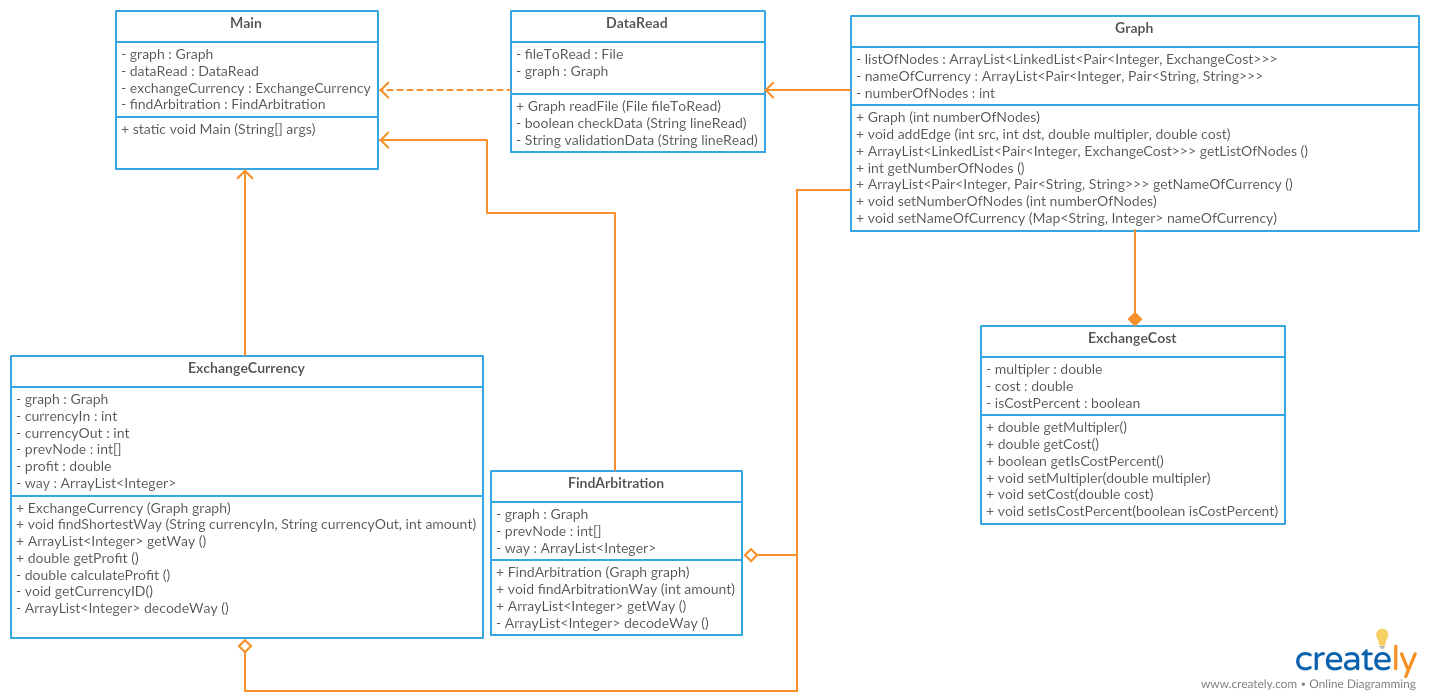
\includegraphics[scale=0.37]{diagram}}
\caption{diagram klas}
\label{fig:diagram2}
\end{figure}

\begin{enumerate}
\item \textbf{Main}
\newline\newline
   Dodane metody:
    \begin{itemize}
        \item \begin{verbatim}private static boolean isAlpha(String name)\end{verbatim}
        metoda używana do sprawdzania, czy podany ciąg znaków zawiera tylko litery. Metoda wykorzystywana podczas wprowadzania danych dotyczących uzyskania najkorzystniejszej ścieżki wymiany walut.
    \end{itemize}
\item \textbf{DataRead}
\newline\newline
   Dodane metody:
   \begin{itemize}
        \item \begin{verbatim}private static boolean isAlpha(String name)\end{verbatim}
        metoda używana do sprawdzania, czy podany ciąg znaków zawiera tylko litery. Metoda wykorzystywana podczas wczytywania danych z pliku,
    \end{itemize}
    \begin{itemize}
    \item \begin{verbatim}private boolean isDouble(String stringToCheck)\end{verbatim}
        metoda używana do sprawdzania, czy podany ciąg znaków zawiera tylko liczby. Metoda wykorzystywana
        podczas wczytywania danych z pliku.
    \end{itemize}
    Zmienione metody:
    \begin{itemize}
        \item \begin{verbatim}private String checkData(String lineRead,
        boolean currencyNameRead, int lineNumber)\end{verbatim}
        metoda oprócz sprawdzenia poprawności danych zajmuje się teraz obsługą błędów związanych z odczytywaniem pliku. Zmiana ta nastąpiła w celu umożliwienia obsługi błędów bez potrzeby wywoływania kolejnych metod.
        \end{itemize}

    Usunięte metody:
    \begin{itemize}
        \item \begin{verbatim}private String validationData (String lineRead)\end{verbatim}
        metoda została usunięta, a jej zadania przejęła metoda checkData.
    \end{itemize}
\item \textbf{Graph}
\newline\newline
   Dodane pola:
   \begin{itemize}
        \item \begin{verbatim}private int numberOfEdges\end{verbatim}
        zmienna przechowująca informację o liczbie krawędzi w grafie, czyli o liczbie kursów walut wczytanych z pliku.
    \end{itemize}
   Zmienione pola:
    \begin{itemize}
        \item \begin{verbatim}private ArrayList<LinkedList<Pair<Integer, ChangeCost>>> listOfNeighbor\end{verbatim}
        zmienna zmieniła nazwę z listOfNodes. Zmiana w celu uzyskania bardziej intuicyjnej nazwy,
    \item \begin{verbatim}private int numberOfVertexes\end{verbatim}
        zmienna zmieniła nazwę z numberOfNodes. Zmiana w celu uzyskania bardziej intuicyjnej nazwy,
    \item \begin{verbatim}private ArrayList<Pair<String, String>> nameOfCurrency\end{verbatim}
        zrezygnowano z reprezentacji zmiennej za pomocą Mapy, na rzecz jej reprezentacji za pomocą ArrayList. Spowodowane jest to usprawnieniem, wedle którego indeks ArrayListy będzie oznaczał ID waluty.
    \end{itemize}
    Dodane metody:
    \begin{itemize}
        \item \begin{verbatim}int getCurrencyID(String shortName)\end{verbatim}
        metoda zwraca ID waluty na podstawie jej skrótu. Metoda dodana w celu uniknięcia implementacji dwóch takich samych metod w klasie odpowiedzialnej za arbitraż oraz za wymianę waluty,
    \end{itemize}
    \begin{itemize}
        \item \begin{verbatim}String getCurrencyShortName(int id)\end{verbatim}
        metoda zwraca skrót waluty na podstawie jej ID. Metoda dodana w celu uniknięcia implementacji dwóch takich samych metod w klasie odpowiedzialnej za arbitraż oraz za wymianę waluty.
    \end{itemize}
    Zmienione metody:
    \begin{itemize}
        \item \begin{verbatim}public Graph(ArrayList<String> listOfCurrency)\end{verbatim}
        argument konstruktora został zmieniony na listę wczytanych walut. Na jej podstawie konsruktor przygotowuje tablicę sąsiedztwa listOfNeighbor oraz zmienną nameOfCurrency. Zmiana wykonana w celu jednoczesnego wypełnienia wyżej wymienionych zmiennych,
    \end{itemize}
    \begin{itemize}
        \item \begin{verbatim}void addEdge(int src, int dst, double multipler, double cost,
        boolean isPercent)\end{verbatim}
        metoda nie zmieniła swojego działania. Został dodany argument, który określa, czy opłata jest stała czy procentowa.
    \end{itemize}
\item \textbf{ChangeCost}
\newline\newline
   Zmienione pola:
    \begin{itemize}
        \item \begin{verbatim}private boolean isPercent\end{verbatim}
        zmienna zmieniła nazwę z isCostPercent,
    \end{itemize}
    Dodane metody:
     \begin{itemize}
    \item \begin{verbatim}ChangeCost(double multipler, double cost, boolean isPercent)\end{verbatim}
        konstruktor stworzony w celu ograniczenia korzystania z metod set(),
    \end{itemize}
\item \textbf{FindArbitration}
\newline\newline
   Dodane pola:
    \begin{itemize}
        \item \begin{verbatim}private double dist[]\end{verbatim}
        zmienna odpowiedzialna za przechowywanie wartości 1/(koszt dotarcia do wierzchołka). Zmienna wprowadzona w celu wykrywania negatywnego cyklu w grafie czyli do znajdowania arbitrażu.
    \end{itemize}
    Zmienione pola:
    \begin{itemize}
    \item \begin{verbatim}private int prevVertex[]\end{verbatim}
        zmienna zmieniła nazwę z prevNode. Zmiana w celu uzyskania bardziej intuicyjnej nazwy.
    \end{itemize}
    Usunięte pola:
     \begin{itemize}
     \item \begin{verbatim}private ArrayList<Integer> way\end{verbatim}
        zmienna, która miała być odpowiedzialna za przechowywanie kolejnych walut należących do arbitrażu. Usunięta z powodu wypisywania elementów arbitrażu wewnątrz metody odpowiedzialnej za jego wyszukiwania.
    \end{itemize}
    Dodane metody:
    \begin{itemize}
     \item \begin{verbatim}private boolean hasCycle(int src, int dst, ChangeCost changeCost)\end{verbatim}
        metoda, która sprawdza czy dany wierzchołek jest częścią negatywnego cyklu czyli, czy dana waluta należy do arbitrażu.
    \end{itemize}
    Zmienione metody:
    \begin{itemize}
     \item \begin{verbatim}double arbitration(int src, double amount)\end{verbatim}
        metoda zmieniła nazwę z findArbitrationWay. Dodatkowo wyszukiwanie arbitrażu rozpoczyna się w konkretnej walucie. Argument ten został dodany, aby znajdować arbitraż nawet w grafach, które nie są połączone.
    \end{itemize}
    Usunięte metody:
    \begin{itemize}
     \item \begin{verbatim}private ArrayList<Integer> findArbitrationWay ()\end{verbatim}
        metoda miała zwracać ścieżkę arbitrażu. Jednak w związku z usunięciem zmiennej odpowiedzialnej za przechowywanie ścieżki, metoda ta stała się bezużyteczna.
    \end{itemize}
\item \textbf{ExchangeCurrency}
\newline\newline
   Dodane pola:
    \begin{itemize}
        \item \begin{verbatim}private double dist[]\end{verbatim}
        zmienna odpowiedzialna za przechowywanie wartości 1/(koszt dotarcia do wierzchołka). Zmienna wprowadzona w celu obliczania odległości między wierzchołkami, czyli w rezultacie do wyliczania końcowego wyniku wymiany.
    \end{itemize}
    Zmienione pola:
    \begin{itemize}
    \item \begin{verbatim}private int prevVertex[]\end{verbatim}
        zmienna zmieniła nazwę z prevNode. Zmiana w celu uzyskania bardziej intuicyjnej nazwy.
    \end{itemize}
    Usunięte pola:
     \begin{itemize}
     \item \begin{verbatim}private int currencyIn\end{verbatim}
        zmienna która miała przechowywać informację o walucie wejściowej. Została usunięta w skutek podawania informacji o walucie wejściowej jako argument metody wyliczającej ścieżkę,
    \end{itemize}
    \begin{itemize}
     \item \begin{verbatim}private int currencyIn\end{verbatim}
        zmienna która miała przechowywać informację o walucie wyjściowej. Została usunięta w skutek podawania informacji o walucie wyjściowej jako argument metody wyliczającej ścieżkę,
    \end{itemize}
    \begin{itemize}
     \item \begin{verbatim}private int profit\end{verbatim}
        zmienna, która miała być odpowiedzialna za przechowywanie końcowego wyniku wymiany walut. Jej zadanie przejęła metoda exchange, która zwraca wynik wymiany,
    \end{itemize}
    \begin{itemize}
     \item \begin{verbatim}private ArrayList<Integer> way\end{verbatim}
        zmienna, która miała być odpowiedzialna za przechowywanie ścieżki wymiany walut. Jej usunięcie spodowane jest jednoczesnym wyliczaniem i wypisywaniem ścieżki w metodzie exchange.
    \end{itemize}
    Zmienione metody:
    \begin{itemize}
     \item \begin{verbatim}double exchange(int src, double amount, int dst)\end{verbatim}
        metoda zmieniła nazwę z findShortestWay. Ponad to, metoda zaczęła wyliczać oraz zwracać wynik wymiany.
    \end{itemize}
    Usunięte metody:
    \begin{itemize}
     \item \begin{verbatim}private double calculateProfit ()\end{verbatim}
        metoda miała zwracać wyliczać wynik wymiany walut. Usunięta z powodu przejęcia jej zadań przez metodę exchange,
    \end{itemize}
    \begin{itemize}
     \item \begin{verbatim}private void getCurrencyID ()\end{verbatim}
        metoda miała zwracać ID waluty na podstawie ich skrótów. Metoda została przeniesiona do klasy Graph,
    \end{itemize}
    \begin{itemize}
     \item \begin{verbatim}private void getCurrencyID ()\end{verbatim}
        metoda miała zwracać ID waluty na podstawie ich skrótów. Metoda została przeniesiona do klasy Graph,
    \end{itemize}
    \begin{itemize}
     \item \begin{verbatim}private ArrayList<Integer> decodeWay ()\end{verbatim}
        metoda miała za zadanie zwracać ścieżkę wymiany walut na podstawie ich ID. Jej zadanie przejęła metoda exchange.
    \end{itemize}
\end{enumerate}

\section{Dodatkowe pakiety nieuwzględnione w specyfikacji implementacyjnej}
\begin{itemize}
\item java.text.DecimalFormat - pakiet odpowiedzialny za zaokrąglanie wyników końcowych
\end{itemize}

\section{Podsumowanie i wnioski}
Program okazał się sporym, choć ciekawym wyzwaniem algorytmicznym. Zastosowany przeze mnie sposób umieszczania i przedstawiania walut w postaci grafu bardzo ułatwił rozwiązanie problemu. Dzięki temu można było użyć algorytmu Bellmana-Forda zarówno do wyszukiwania arbitrażu jak i do znalezienia najkorzystniejszej ścieżki wymiany waluty.
\newline\newline
Po zrealizowaniu tego projektu doszedłem do wniosku, że wyszukiwanie najkorzystniejszej ścieżki wymiany waluty można było zrealizować algorytmem DFS. Pozwoliłoby to na uzyskanie bardziej precyzyjnych danych.
\newline\newline
Realizując ten projekt wiele się nauczyłem. Popełniłem też sporo błędów, a co za tym idzie, wyciągnąłem sporo wniosków. Dzięki temu będę wiedział w jaki sposób realizować projekty w przyszłości.

\end{document}
